%!TEX root=paper/paper.tex
\chapter{Introduction}\label{sec:introduction}

\PM{Perception}
It is a well-known fact that human perception is Anytime, meaning that a scene can be described after even a short presentation.
Perception is also progressive, meaning that the quality of description increases with more time.
The progressive time course of visual perception has been confirmed by multiple studies \parencite{Vanrullen-1996,Fei-Fei-Vision-2007}, and some studies have also provided evidence that such progressive enhancement occurs in an ontologically meaningful way.
For example, people tend to recognize something as an animal before recognizing it as a dog \parencite{Mace-PloS-2009}.
The underlying mechanisms of this behavior are unknown, and only a few attempts have been made to explain the temporal dynamics.
For instance, a promising work has employed the framework of sequential decision processes \parencite{Hegde-Neuro-2008}.

\PM{Applications}
Meanwhile, automated visual recognition has achieved levels of performance that allow useful real-world implementation.
As recognition methods are applied at scale, managing their resource (power or cpu-time) cost becomes increasingly important.
For tasks such as personal robotics, it is crucial to be able to deploy varying levels of processing to different stimuli, depending on computational demands on the robot.
However, state-of-the-art methods tend to be computationally expensive and insensitive to Anytime demands.

\PM{Case Study}
A hypothetical system for vision-based advertising presents another example: companies pay money to have their products detected in images on the internet.
The system has different values (in terms of cost per click) and accuracies for different classes of objects, and the queue of unprocessed images varies in size.
The recognition strategy to maximize profit in such an environment has to exploit every signal available to it if there is not enough time to run detection for all classes.
The quality of the detections could be Anytime, depending on the length of the queue (lowering recall when queue pressure grows).

\PM{Features}
For most state-of-the-art classification methods, different features are extracted from an image instance at different costs, and contribute differently to decreasing classification error.
Although it can generally be truthfully said that ``the more features, the better,'' high accuracy can of course be achieved with only a small subset of features for some instances.
Additionally, different instances benefit from different subsets of features.
For example, simple binary features are sufficient to quickly detect faces \parencite{Viola-IJCV-2004} but not more varied visual objects, while the features most useful for separating landscapes from indoor scenes \parencite{Xiao-CVPR-2010} are different from those most useful for recognizing fine distinctions between bird species \parencite{Farrell-ICCV-2011}.
\autoref{fig:features} presents some common visual features.

%!TEX root=paper/paper.tex
\begin{figure}[ht]
\centering
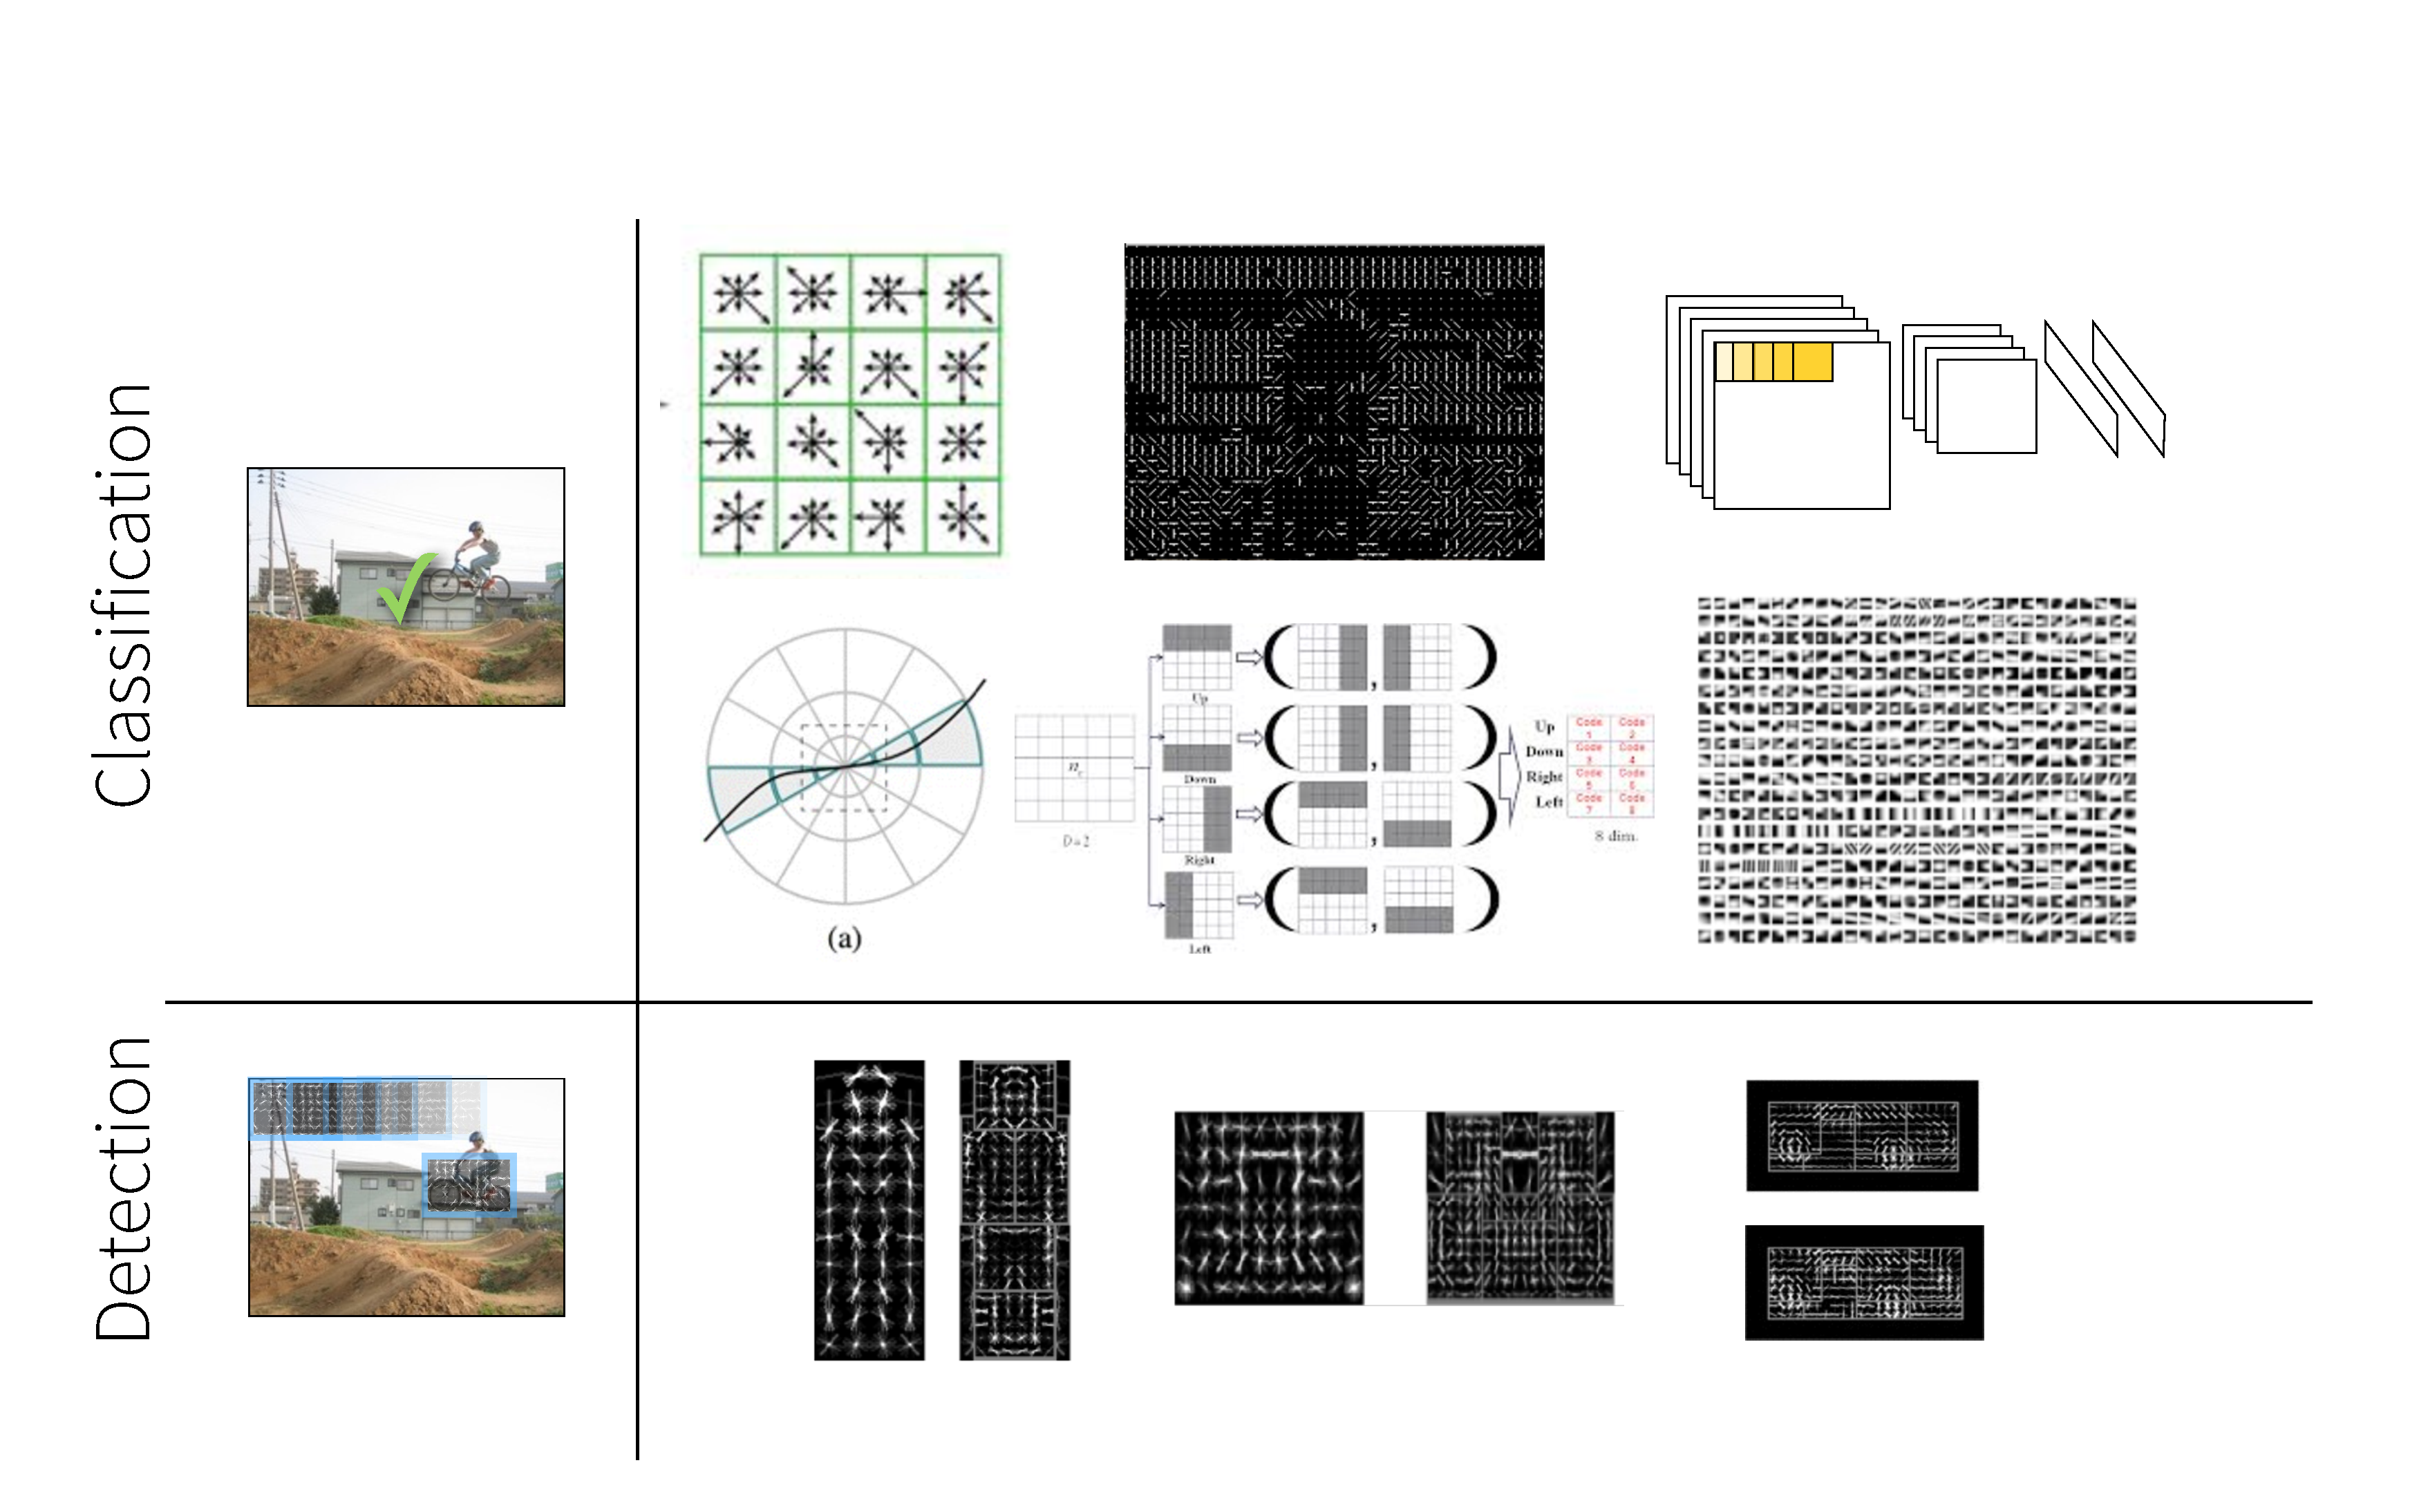
\includegraphics[width=\linewidth]{../../figures/features.pdf}
\caption[Summary of the variety of features for object detection and classification.]{
Summary of the variety of features for object detection and classification.
In reading order for classification: SIFT \parencite{Lowe2004}, HOG \parencite{Dalal2005}, CNN \parencite{Krizhevsky-NIPS-2012}, Self-Similarity \parencite{Shechtman2007}, Haar basis functions \parencite{Viola-IJCV-2004}, basis functions learned with sparse coding \parencite{Olshausen1996}.
In reading order for detection: person, bicycle, and car templates for the Deformable Part Model \parencite{Felzenszwalb2010a}.
}\label{fig:features}
\end{figure}


\PM{Detection}
State-of-the-art object detectors are slow, and need to process many regions of each image \parencite{Felzenszwalb2010a}.
This is true even for recent approaches based on Convolutional Neural Networks (CNNs) \parencite{Girshick-CVPR-2014}.
While convolutional models are efficient to implement due to the availability of high-performance primitives, the amount of work to perform complete inference at all candidate region windows is still considerable.
To maximize early performance gains, scene and inter-object contextual cues can be exploited in two ways.
First, detectors can be ordered according so as to maximize the chance of finding objects actually present in the image.
Second, regions can be processed in an intelligent order, with most likely locations selected first.

\PM{Costliness}
Computing all features, running all detectors, or processing all regions for all images is infeasible in a deployment sensitive to Anytime needs, as each feature brings a significant computational burden.
Yet the conventional approach to evaluating visual recognition does not consider efficiency, and evaluates performance independently across classes.
We address the problem of selecting and combining a subset of features under an Anytime cost budget, specified in terms of wall time or total power expended or another metric, and propose a new \emph{costliness} measure of performance vs. cost.

\PM{Our Approach}
To exploit the fact that different instances benefit from different subsets of features, our approach to feature selection is a sequential policy.
To learn the policy parameters, we formulate the problem as a Markov Decision Process (MDP) and use reinforcement learning methods.
The method does not make many assumptions about the underlying actions, which can be existing object detectors and feature-specific classifiers.
With different settings of parameters, we can learn policies ranging from \textbf{Static, Myopic}---greedy selection not relying on any observed feature values, to \textbf{Dynamic, Non-myopic}---relying on observed values and considering future actions.

\PM{Detection}
For detection, the actions are time-consuming detectors applied to the whole image, as well as a quick scene classifier.
We run scene context and object class detectors over the whole image sequentially, using the results of detection obtained so far to select the next actions.
Since the actions are time-consuming, we use a powerful inference mechanism to select the best next action.
We evaluate on the PASCAL VOC dataset and obtain better performance than all baselines when there is less time available than is needed to exhaustively run all detectors.

\PM{Classification}
Classification actions are much faster than detectors, and the action-selection method accordingly needs to be fast.
Because different features can be selected for different instances, and because our system may be called upon to give an answer at any point during its execution, the feature combination method needs to be robust to a large number of different observed-feature subsets.
To this end, we consider several value-imputation methods, and present a method for learning several classifiers for different clusters of observed-feature subsets.
We first demonstrate on synthetic data that our algorithm learns to pick features most useful for the specific test instance.
We demonstrate the advantage of non-myopic over greedy, and of dynamic over static on this and the Scene-15 visual classification dataset.
Then we show results on a subset of the hierarchical ImageNet dataset, where we additionally learn to provide the most specific answers for any desired cost budget and accuracy level.

\PM{Cascaded CNN}
We additionally investigate a novel approach for speeding up a state-of-the-art CNN-based detection method, and propose a general technique for accelerating CNNs applied to class imbalanced data.
We bring the classic idea of the cascade to CNNs by inserting a \emph{reject} option between CNN layers.
When the CNN processes batches of images, which is standard for many applications, the reject layers allows the CNN to ``thin'' the batch as it progresses through the network, thus saving processing time.
We also consider a variety of strong baselines for speeding up R-CNN.
On the PASCAL VOC dataset, the Cascaded CNN method obtains nearly the state-of-the-art performance of \cite{Girshick-CVPR-2014} with a 8x speed-up.
